% Thanks to http://tex.stackexchange.com/a/30782/5645 for this
% example!
\documentclass{article}
\usepackage{amsmath}
\usepackage{mathptmx}
\usepackage{tikz}
\usepackage{pgfplots}
\usepackage{tkz-fct}
\usetikzlibrary{angles, quotes}
\usetikzlibrary{arrows.meta, arrows}
\usetikzlibrary{external}
\tikzexternalize[prefix={external/}]

\tikzset{
    export as png/.style={
        external/system call/.add={}{
            && convert -density #1 -transparent white "\image.pdf" "\image.png"
        },
    },
    export as png/.default={200},
}

\DeclareSymbolFont{symbolsb}{OMS}{cmsy}{m}{n}
\SetSymbolFont{symbolsb}{bold}{OMS}{cmsy}{b}{n}
\DeclareSymbolFontAlphabet{\mathcal}{symbolsb}
\definecolor{myblue}{rgb}{0.067,0.529,0.871}
\definecolor{mypurple}{rgb}{0.859,0.071,0.525}
\definecolor{myred}{rgb}{1.0, 0.13, 0.32}
\definecolor{mygreen}{rgb}{0.01, 0.75, 0.24}
\definecolor{myblack}{gray}{0.5}
\definecolor{mygray}{gray}{0.7}

\def\req{\protect\rotatebox{90}{$\scriptstyle=$}}

\begin{document}

\tikzset{export as png}

\tikzsetnextfilename{sumas-riemann-positivas-negativas}
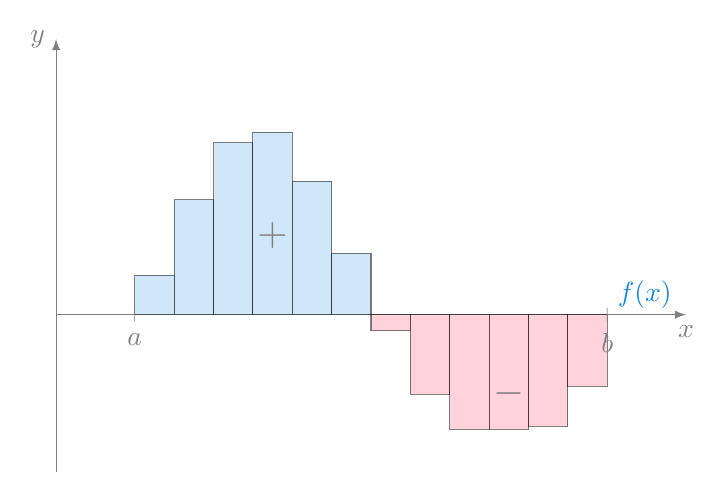
\begin{tikzpicture}[scale=1]
    \tkzInit[xmax=7.5, ymin=-2, ymax=3, ystep=1]
    \tkzDrawY[noticks, color=myblack]
    \tkzDrawX[noticks, color=myblack]
    \tkzFct[line width=1pt, color = myblue, domain = 1:7]{2*sin(\x-1)+0.5}
    \tkzDefPointByFct(7) \tkzGetPoint{A} 
    \tkzLabelPoint[above right, color=myblue](A){$f(x)$}
    \tkzDrawRiemannSumInf[fill=myblue!40, interval=1:4, number=6]
    \tkzDrawRiemannSumInf[fill=myred!40, interval=4:7, number=6]
    \tkzFct[line width=1pt, color = myblue, domain = 1:7]{2*sin(\x-1)+0.5}
    \tkzText[color=myblack](1,0){\tiny $|$}
    \tkzText[below, color=myblack](1,-0.1){$a$}
    \tkzText[color=myblack](7,0){\tiny $|$}
    \tkzText[below, color=myblack](7,-0.1){$b$}
    \tkzText[color=myblack](2.75,1){\Large $+$}
    \tkzText[color=myblack](5.75,-1){\Large $-$}
\end{tikzpicture}
\end{document}


